% Indicate the main file. Must go at the beginning of the file.
% !TEX root = ../main.tex

%----------------------------------------------------------------------------------------
% CHAPTER TEMPLATE
%----------------------------------------------------------------------------------------


\chapter{Resultate} % Main chapter title

\label{Chapter4} % Change X to a consecutive number; for referencing this chapter elsewhere, use \ref{ChapterX}

%----------------------------------------------------------------------------------------
% SECTION 1
%----------------------------------------------------------------------------------------

\subsection{Ergebnisse der Churn-Analyse}

Die initiale Auswertung zeigte, dass der durchschnittliche Churn-Wert in den PM2-Projekten deutlich variiert. Einzelne Pull Requests wiesen einen sehr hohen Churn auf (über 1000 Zeilen geändert), während viele Änderungen im Bereich von 10 bis 50 Zeilen lagen. 

Die Datenanalyse ergab folgende Erkenntnisse:

\begin{itemize}
    \item \textbf{Korrelation:} Es konnte keine Korrelation zwischen dem Churn und der PR-Latenz festgestellt werden.
    \item \textbf{Ausreisser:} Besonders umfangreiche Pull Requests führten teilweise zu aussergewöhnlich langen Latenzzeiten, was sich als typische Herausforderung im Code Review Prozess darstellt.
    \item \textbf{Review-Aktivität:} Pull Requests mit geringem Churn wurden häufig schneller bearbeitet, was die Hypothese unterstützt, dass kleinere Changes leichter zu prüfen sind.
    \item \textbf{Kein Unterschied zwischen den Klassen:} Es lässt sich kein wesentlicher Unterschied zwischen der Teilzeit- und der Vollzeitklasse feststellen.    
\end{itemize}

Die Ergebnisse der Scatterplots verdeutlichen diese Tendenzen. In Abbildung \ref{fig:pr-latency-churn-added-plus-deleting} ist die Korrelation grafisch dargestellt.


\begin{figure}[th]
\centering
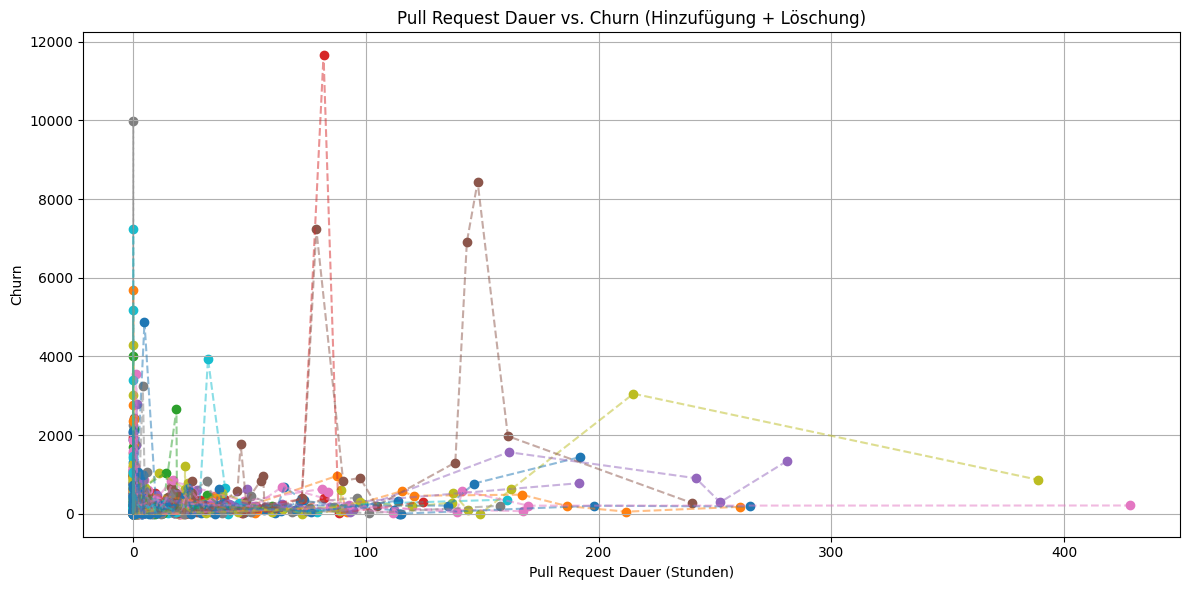
\includegraphics[width=\textwidth]{Figures/pr-latency-churn.png}
\decoRule
\caption{Scatterplot der Churn-Werte in Relation zur PR-Latenz}
\label{fig:pr-latency-churn-added-plus-deleting}
\end{figure}


Zusammenfassend liefert das erste Experiment Hinweise darauf, dass ein erhöhter Churn tatsächlich mit einer höheren PR-Latenz einhergeht. Um diese Hypothese jedoch weiter zu festigen, sind weitere Analysen und statistische Tests notwendig, die im nächsten Kapitel beschrieben werden.

%-----------------------------------
% SUBSECTION 2 (optional)
%-----------------------------------

\subsection{Fazit des ersten Experiments}

Das Experiment zur Churn-Metrik bildete die Grundlage für unsere weiteren Analysen. Es zeigte sich, dass in den studentischen Projekten ähnliche Muster auftreten wie in professionellen Softwareentwicklungsprozessen, was die Relevanz und Generalisierbarkeit der Untersuchung unterstreicht.